\documentclass[11pt]{article}
\usepackage{amsmath, amssymb, amsthm}
\usepackage{geometry}
\usepackage{hyperref}
\usepackage{tikz}
\usetikzlibrary{arrows.meta, positioning}
\geometry{margin=1in}

\title{Notes 00 \\ Review of Statistics: \\ Generalized Linear Models (GLMs)}
\author{DATA 000: Advanced Computational Methods in Education and the Social Sciences}
\date{Alexander \\ Spring 2026}

\begin{document}

\maketitle

\tableofcontents

\section{Introduction}

\textbf{Generalized Linear Models (GLMs)} are a flexible extension of linear regression that allow us to model response variables that are not normally distributed, such as binary outcomes (pass/fail), counts (number of events), or proportions\ [2][5][6][7]. GLMs are widely used in education, social sciences, public health, and data science.

\section{GLM Framework and Components}

A GLM has three key components\ [2][4][6]:

\begin{enumerate}
    \item \textbf{Random Component:} Specifies the probability distribution of the response variable $Y$ (e.g., normal, binomial, Poisson).
    \item \textbf{Systematic Component:} Linear predictor $\eta = \beta_0 + \beta_1 X_1 + \cdots + \beta_p X_p$.
    \item \textbf{Link Function:} Connects the mean of the response variable ($\mu = E[Y]$) to the linear predictor: $g(\mu) = \eta$.
\end{enumerate}

\subsection*{Visualization: GLM Structure}
\begin{center}
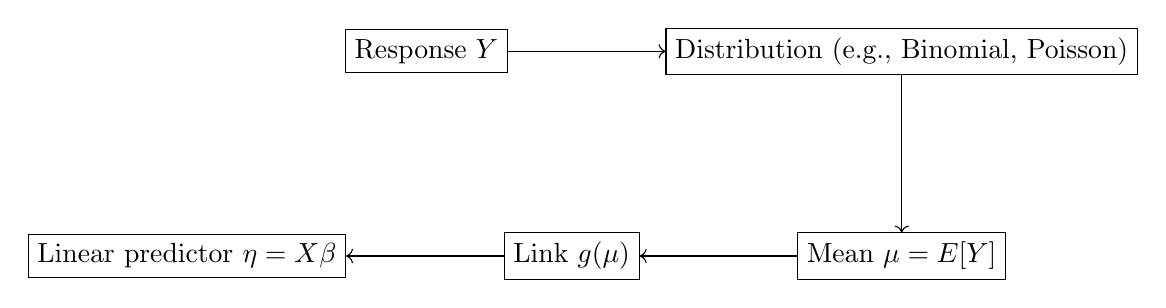
\begin{tikzpicture}[node distance=2cm]
  \node (y) [draw, rectangle] {Response $Y$};
  \node (dist) [right=of y, draw, rectangle] {Distribution (e.g., Binomial, Poisson)};
  \node (mean) [below=of dist, draw, rectangle] {Mean $\mu = E[Y]$};
  \node (link) [left=of mean, draw, rectangle] {Link $g(\mu)$};
  \node (lp) [left=of link, draw, rectangle] {Linear predictor $\eta = X\beta$};
  \draw[->] (y) -- (dist);
  \draw[->] (dist) -- (mean);
  \draw[->] (mean) -- (link);
  \draw[->] (link) -- (lp);
\end{tikzpicture}
\end{center}

\section{Link Functions and Distributions}

The choice of link function and distribution depends on the nature of the response variable\ [2][5][6]:

\begin{tabular}{|l|l|l|}
\hline
\textbf{Outcome Type} & \textbf{Distribution} & \textbf{Link Function} \\
\hline
Continuous (unbounded) & Normal & Identity: $g(\mu) = \mu$ \\
Binary (0/1) & Binomial & Logit: $g(\mu) = \log\left(\frac{\mu}{1-\mu}\right)$ \\
Counts (0,1,2,...) & Poisson & Log: $g(\mu) = \log(\mu)$ \\
Proportions (0-1) & Binomial & Logit or Probit \\
Positive, skewed & Gamma & Log or Inverse \\
\hline
\end{tabular}

\subsection*{Visualization: Common Link Functions}
\begin{center}
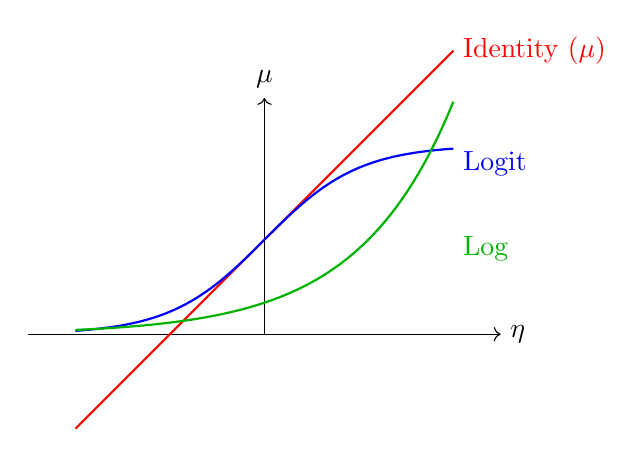
\begin{tikzpicture}[scale=1.2]
  % x-axis
  \draw[->] (-2.5,0) -- (2.5,0) node[right] {$\eta$};
  % y-axis
  \draw[->] (0,0) -- (0,2.5) node[above] {$\mu$};
  % Identity link
  \draw[red, thick, domain=-2:2] plot (\x,{\x+1});
  \node[red, right] at (2,3) {Identity ($\mu$)};
  % Logit link
  \draw[blue, thick, domain=-2:2, samples=100] plot (\x,{2/(1+exp(-2*\x))});
  \node[blue, right] at (2,1.8) {Logit};
  % Log link
  \draw[green!70!black, thick, domain=-2:2, samples=100] plot (\x,{exp(\x)/3});
  \node[green!70!black, right] at (2,0.9) {Log};
\end{tikzpicture}
\end{center}

\section{GLMs in Practice: Examples}

\subsection{Poisson Regression (Counts)}

\textbf{Purpose:} Model count data (e.g., number of events, absences, incidents).

\textbf{Model:}
\[
Y \sim \text{Poisson}(\mu), \quad \log(\mu) = \beta_0 + \beta_1 X_1 + \cdots + \beta_p X_p
\]

\subsection*{Example: Education (with Solution)}

\textbf{Scenario:} A principal wants to model the number of absences ($Y$) per student as a function of distance from school ($X$ in miles):

\[
\log(\mu) = 1.2 + 0.3 X
\]

\textbf{Interpretation:}
- For each additional mile from school, the log expected absences increases by 0.3.
- The expected number of absences for a student living 2 miles away:
\[
\log(\mu) = 1.2 + 0.3 \times 2 = 1.8 \implies \mu = e^{1.8} \approx 6.05
\]

\subsection*{Visualization: Poisson Mean Curve}
\begin{center}
\begin{tikzpicture}[scale=1.1]
  \draw[->] (0,0) -- (4.5,0) node[right] {Distance (miles)};
  \draw[->] (0,0) -- (0,7) node[above] {Expected Absences};
  \draw[thick, domain=0:4, samples=100] plot (\x,{exp(1.2+0.3*\x)});
  \foreach \x in {0,1,2,3,4} {
    \draw[dashed] (\x,0) -- (\x,{exp(1.2+0.3*\x)});
    \filldraw[blue] (\x,{exp(1.2+0.3*\x)}) circle (2pt);
  }
\end{tikzpicture}
\end{center}

\subsection{Logistic Regression (Binary Outcomes)}

\textbf{Purpose:} Model probability of a binary outcome (e.g., pass/fail, yes/no).

\textbf{Model:}
\[
Y \sim \text{Binomial}(n, p), \quad \log\left(\frac{p}{1-p}\right) = \beta_0 + \beta_1 X_1 + \cdots + \beta_p X_p
\]

\subsection*{Example: Social Science (with Solution)}

\textbf{Scenario:} Predicting whether a respondent supports a new policy ($Y=1$) based on years of education ($X$):

\[
\log\left(\frac{p}{1-p}\right) = -1 + 0.2 X
\]

\textbf{Interpretation:}
- Each additional year of education increases the log odds of supporting the policy by 0.2.
- For $X=8$ years:
\[
\log\left(\frac{p}{1-p}\right) = -1 + 0.2 \times 8 = 0.6
\]
\[
\frac{p}{1-p} = e^{0.6} \approx 1.82 \implies p = \frac{1.82}{1+1.82} \approx 0.65
\]

\subsection*{Visualization: Logistic Curve}
\begin{center}
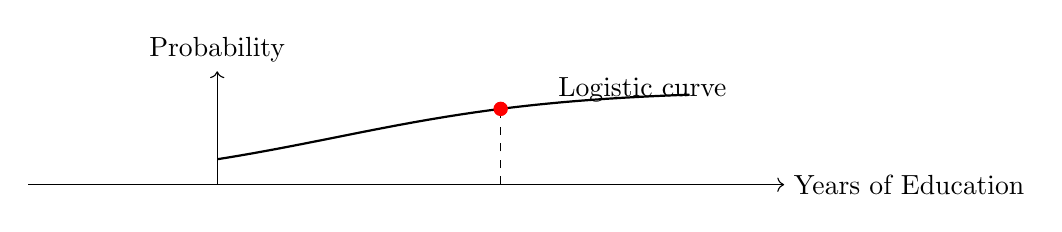
\begin{tikzpicture}[scale=1.2]
  \draw[->] (-2,0) -- (6,0) node[right] {Years of Education};
  \draw[->] (0,0) -- (0,1.2) node[above] {Probability};
  \draw[thick, domain=0:5, samples=100] plot (\x,{1/(1+exp(-(-1+0.8*\x)))});
  \node at (4.5,1) {Logistic curve};
  \draw[dashed] (3,0) -- (3,{1/(1+exp(-(-1+0.8*3)))});
  \filldraw[red] (3,{1/(1+exp(-(-1+0.8*3)))}) circle (2pt);
\end{tikzpicture}
\end{center}

\section{Fitting GLMs and Interpretation}

\begin{itemize}
    \item Parameters ($\beta$) are usually estimated by \textbf{maximum likelihood}.
    \item Interpretation depends on the link function:
        \begin{itemize}
            \item \textbf{Logit:} Coefficients are in log odds; exponentiate for odds ratios.
            \item \textbf{Log:} Coefficients are in log counts; exponentiate for rate ratios.
        \end{itemize}
    \item Model fit can be assessed with deviance, AIC, pseudo-$R^2$, and residual plots.
    \item GLMs can include interaction terms and categorical predictors (via dummy variables).
\end{itemize}

\section{When to Use GLMs}

\begin{itemize}
    \item When the response variable is not normally distributed (e.g., binary, count, proportion).
    \item When the relationship between predictors and the mean of the response is not linear.
    \item When you need to model rates, probabilities, or counts.
    \item In education, social sciences, health, insurance, and many other fields\ [5][8].
\end{itemize}

\section{Summary Table: GLMs and Links}

\begin{tabular}{|l|l|l|l|}
\hline
\textbf{Model} & \textbf{Distribution} & \textbf{Link} & \textbf{Typical Outcome} \\
\hline
Linear regression & Normal & Identity & Continuous \\
Logistic regression & Binomial & Logit & Binary \\
Poisson regression & Poisson & Log & Count \\
Gamma regression & Gamma & Log/Inverse & Positive, skewed \\
\hline
\end{tabular}

\section{Further Notes}

\begin{itemize}
    \item GLMs generalize linear regression and allow for a much wider range of data modeling\ [2][5][6][7].
    \item Choosing the right link and distribution is crucial for valid inference.
    \item Always check model diagnostics and fit.
\end{itemize}

\end{document}
